\section{ESTADO DEL ARTE}

En este capítulo se explora el estado del arte del uso de imágenes satelitales en diversas áreas y las técnicas
de análisis relevantes para este proyecto. Esta investigación tiene el fin de entender la forma en que se aplican en sus
diversos campos de aplicación y cuáles técnicas son las más eficaces en el campo a estudiarse.

En particular, los temas a desarrollarse son una revision del estado de la teledetección y los recursos disponibles, las
bases de las redes neuronales convolucionales y su uso en el análisis de imágenes satelitales, las técnicas modernas en
uso en la investigación y en aplicaciones en el mundo real.

\subsection{Teledetección}

Teledetección se refiere a la captación o detección remota de alguna señal o imagen. En este contexto nos referimos
específicamente a imágenes captadas por medio de un sensor montado en un satélite artificial o algún vehículo aéreo
como un avión o un dron, para extraer información. Estas imágenes contienen información multiespectro, es decir, además
de la luz visible se toman imágenes de bandas invisibles como por ejemplo la luz infrarroja.
\autocite{globalforestlink-how-sat-imaging-work} A lo largo de este proyecto, el término \enquote{teledetección} se
refiere a la captación de imágenes por medio de satélites.

Para la captura de estas imágenes se emplean varios métodos, que se dividen en dos categorías: sensores pasivos
recolectan radiación electromagnética reflejada del sol, mientras que sensores activos emiten su propia radiación y
captan la reflexión de la tierra. Sensores pasivos requieren de una cantidad importante de energía para operar, pero
tienen la ventaja de operar a cualquier hora del día y la capacidad de crear imágenes en bandas que el sol no emite.
\autocite{globalforestlink-how-sat-imaging-work}

Los primeros programas de observación de la tierra por medio de satélites surgieron en los años 70 y 80. El primero fue
el programa Landsat de los Estados Unidos en 1972, y le siguieron programas similares en India, Francia y la Unión
Europea. \autocite{esa-space-year-2007}

\begin{figure}
    \centering
    \subfloat[\centering Cámara digital normal]{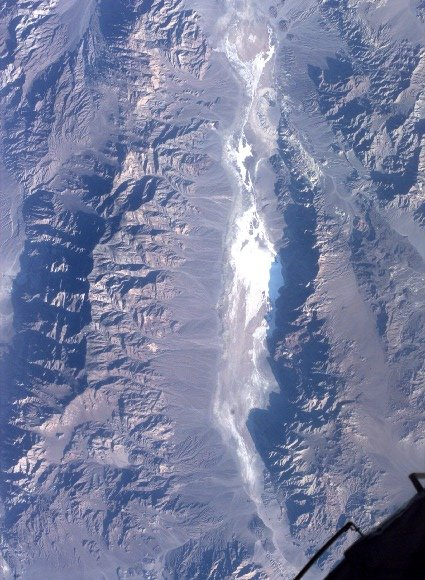
\includegraphics[width=0.275\textwidth]{img/Death_Valley_from_space.JPG}}
    \qquad
    \subfloat[\centering Radar de Apertura Sintética]{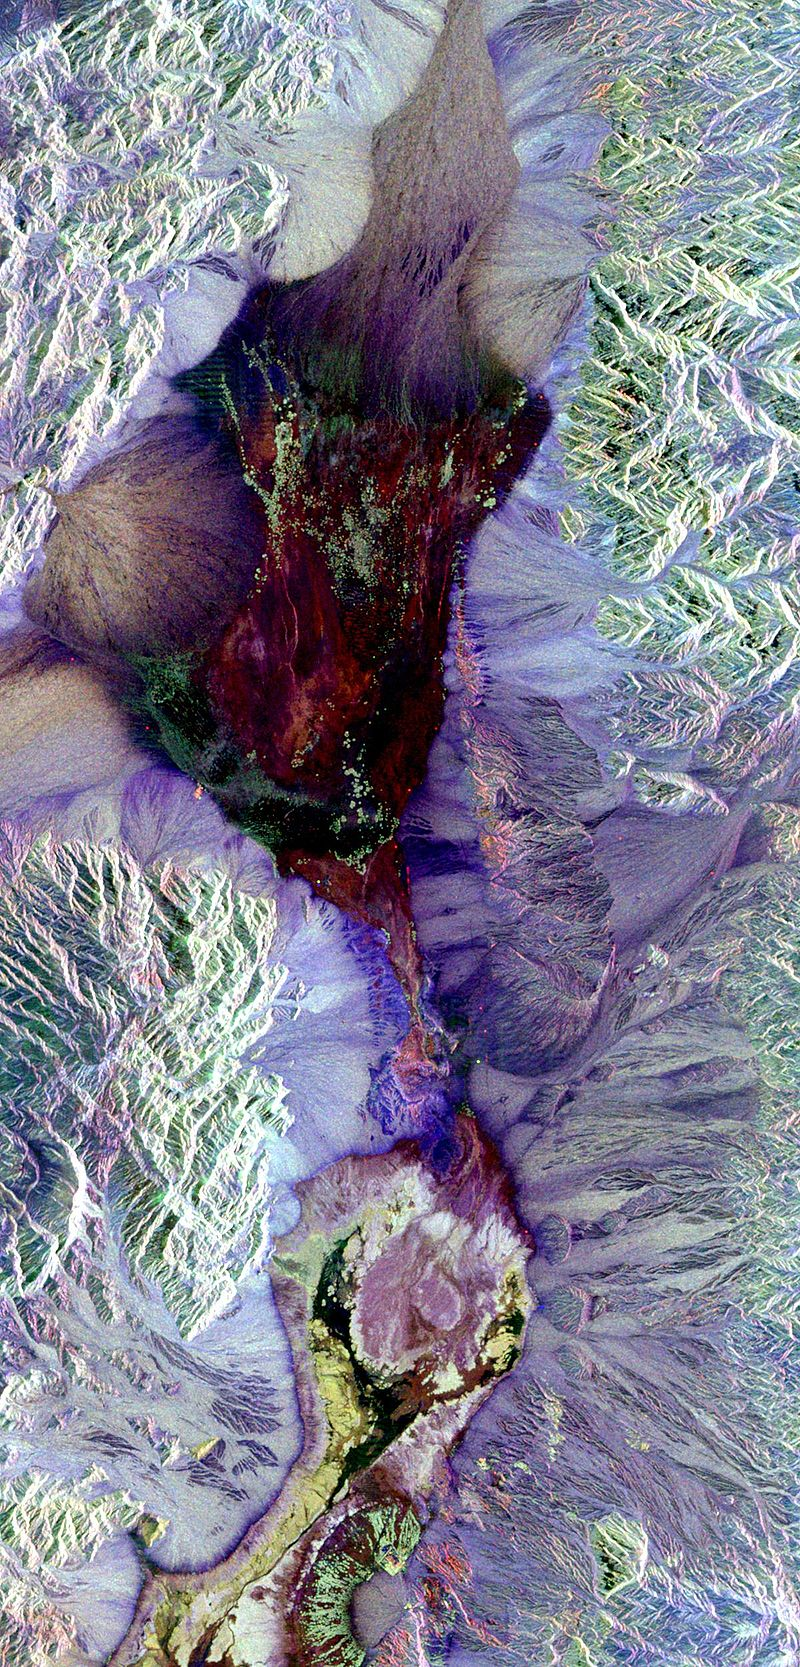
\includegraphics[width=0.175\textwidth]{img/800px-Death-valley-sar.jpg}}
    \caption{Imágenes satelitales del Valle de la Muerte con diferentes resoluciones espectrales. El área superior de (a)
    coincide con el área inferior de (b).}
    \label{fig:1}
\end{figure}

\subsubsection{Aplicaciones}

Imágenes satelitales proveen información muy útil para todo tipo de estadísticas en áreas relacionadas con el
territorio, como por ejemplo la agricultura, silvicultura y el estudio de uso del suelo. El estudio de la agricultura a
gran escala por medio de la teledetección se realizó por primera vez entre 1974 y 1977 por medio de datos de Landsat 1,
a cargo de la NASA, la Oficina Nacional de Administración Oceánica y Atmosférica (NOAA) y el Departamento de
Agricultura de los Estados Unidos (USDA). \autocite{allen-usda-study}

Dado que las imágenes producidas generalmente cubren toda o casi toda el área de estudio, y que suelen ser
multiespectrales, lo que provee datos que fotografías ordinarias no contienen, cualquier aplicación que involucre
estudiar un área vasta puede beneficiarse de ellas. Dependiendo de la resolución, aplicaciones que involucren detalles
más finos también las pueden aprovechar, como por ejemplo su uso en aplicaciones de mapas digitales.

\subsubsection{Características de los datos}

La calidad de imágenes recolectadas por teledetección se mide de cuatro formas, estas son su resolución espacial,
espectral, radiométrica y temporal.

{\bf Resolución espacial}: el tamaño de un píxel en una imagen rasterizada. Típicamente corresponde a un área cuadrada
de entre 1 y 1000 $m^2$.

{\bf Resolución espectral}: la longitud de onda de las diferentes bandas de frecuencia capturadas, normalmente
relacionada a la cantidad de bandas de frecuencia. El sensor Hyperion en \enquote{Earth Observing-1}, por ejemplo,
observa 220 bandas entre 0,4 y 2,5 $\mu m$, con una resolución espectral de 0,10--1.11 $\mu m$ por
banda. \autocite{earth-observatory-earth-observing-1} En imágenes de espectros no visibles, la visualización se hace
con colores falsos, en donde cada banda es asignada un color visible. Un ejemplo se ve en la figura \ref{fig:1}.

{\bf Resolución radiométrica}: la cantidad de niveles de intensidad de radiación detectable por el sensor. Típicamente
entre 8 y 14 bits de información, correspondiente a 256 a 16384 niveles en cada banda. La cantidad de ruido en el
sensor también afecta la resolución radiométrica.

{\bf Resolución temporal}: la cantidad de sobrevuelos del avión o satélite, importante solamente cuando se realizan
series de tiempo, promedios o mosaicos, como por ejemplo en el monitoreamiento de la agricultura.

\begin{figure}
    \centering
    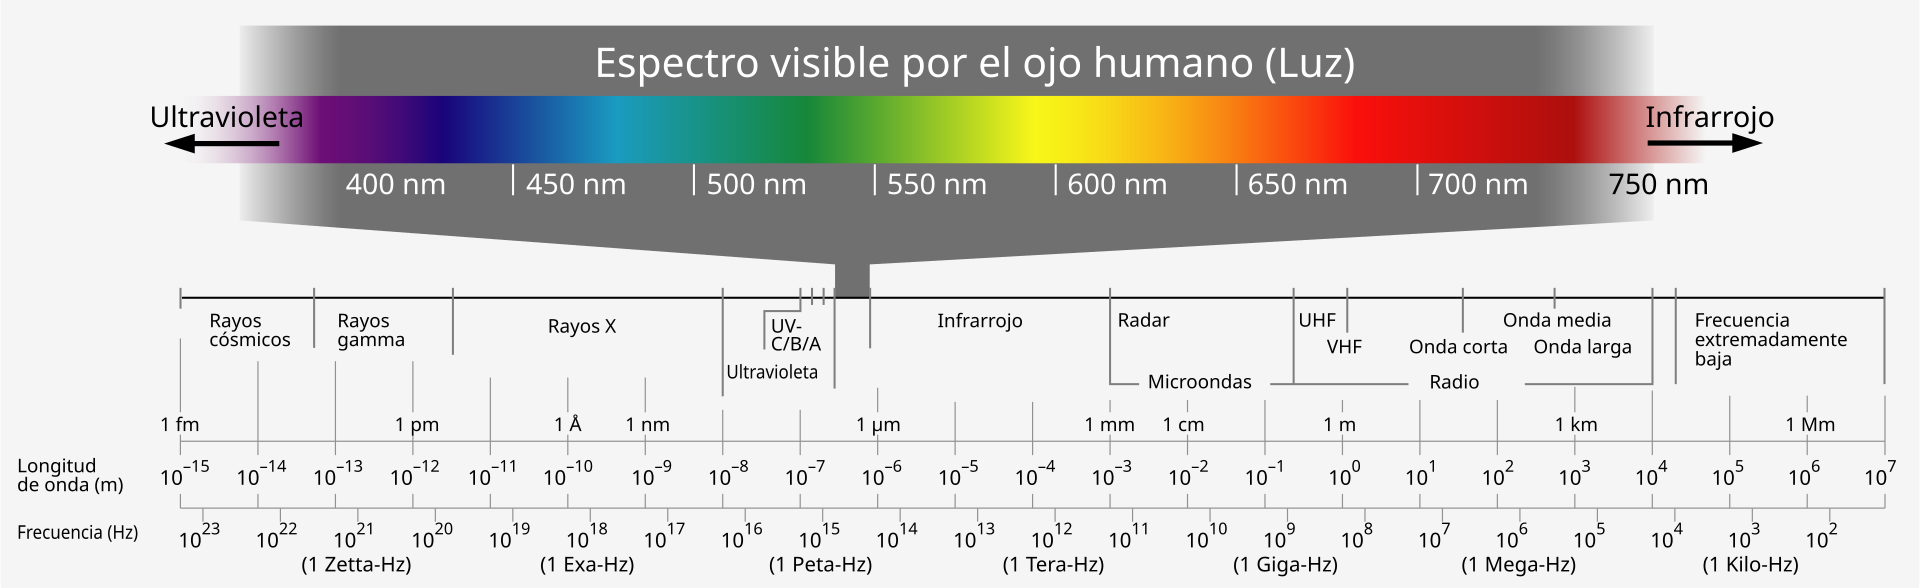
\includegraphics[width=0.9\textwidth]{img/Electromagnetic_spectrum-es.svg.png}
    \caption{Espectro electromagnético visualizado. Diferentes sustancias y materiales reflejan una variedad de
    frecuencias más allá del espectro visible, que es relativamente reducido.}
    \label{fig:3}
\end{figure}

\subsubsection{Disponibilidad de recursos}

Existen varios repositorios de datos de teledetección disponibles para usos comerciales como académicos. Los programas
de observación terrestre de la NASA y de la ESA, Landsat y Copernicus respectivamente, disponibilizan recursos por
medio de portales en la internet. Para los datos de Landsat, uno de los recursos más accesibles es Google Earth Engine,
que permite el procesamiento de imágenes en línea, de forma gratuita para usos no comerciales.
\autocite{landsat-data-access} El programa Copernicus por otro lado provee un navegador de imágenes, una forma de
descargar datos con algunos filtros, y todo esto de forma gratuita tanto para fines académicos como comerciales.
\autocite{copernicus-licences} También ofrecen un espacio de trabajo en línea, similar en propósito a Google Earth
Engine. \autocite{copernicus-ds-about}


\subsection{Redes Neuronales Convolucionales}

Una Red Neuronal Convolucional (o CNN por sus siglas en inglés) es un tipo de red neuronal artificial en la cual las
neuronas procesan datos de entrada por medio de filtros de convolución. Esto implica el procesamiento de un grupo de
datos cercanos, lo que permite interpretar el contexto de un dato, en contraste con redes neuronales típicas. Esta
propiedad hace que las CNN sean el método preferido para el procesamiento de imágenes por medio de redes neuronales.
\autocite{hands-on-machine-learning} \autocite{ciresan-cnn}

Este método de procesamiento permite procesar una gran cantidad de entradas con una cantidad reducida de neuronas,
comparado con una red neuronal típica con la misma capacidad.

Por ejemplo, considerando una red neuronal con una capa de entrada y una capa siguiente con la misma cantidad de
neuronas $N$ en ambas, una red neuronal densa, es decir donde cada neurona de una capa está conectada a cada neurona de
la siguiente capa, contiene $N \times N$ conexiones. En contraste, una red neuronal convolucional equivalente estaría
compuesta de tan solo $N$ neuronas, mientras que al mismo tiempo captura un grupo de píxeles en cada neurona en lugar
de uno solo.

Para el procesamiento se utilizan los filtros de convolución, matrices de dimensiones reducidas comparadas con la
imagen, cuyas celdas contienen coeficientes. Este filtro se superpone sobre una sección de la imagen, y los valores de
los píxeles se multiplican con los de la celda superpuesta del filtro, y la suma de los productos es el resultado de la
convolución del grupo de píxeles. Con una representación adecuada de los datos de cada píxel, estos filtros, también
llamados {\it kernels }, pueden usarse en la detección de bordes en cualquier orientación, reducción de ruido,
aumentación de intensidad de píxeles de cierto color o brillo, entre otros. \autocite{ciresan-cnn}

\subsubsection{Aplicaciones}

CNN ya se han utilizado en todo tipo de aplicaciones relacionadas con imágenes y videos, entre ellas clasificación de
imágenes, segmentación de imágenes, detección de objetos e inclusive en análisis de imágenes de inundación para
predecir la gravedad de uno de estos tipos de desastre natural. \autocite{pally2022105285}

También se ha usado extensivamente en aplicaciones relacionadas a la teledetección, con una gran colección de técnicas,
conjuntos de datos, material de aprendizaje y software de libre acceso en artículos web, videos y repositorios de
código. \autocite{tds-landuse-classification} \autocite{repo-satellite-image-dl} Queda claro que los modelos
convolucionales son muy eficaces en el procesamiento de imágenes, y la cantidad de material estudiado relacionado a las
imágenes satelitales facilitaría enormemente la aplicación en el tema de este proyecto.

\subsubsection{Técnicas y arquitecturas}

